\documentclass[10pt, twocolumn]{article}

%math
\usepackage{amsmath}
\usepackage{amssymb}
\usepackage{mathtools}
%logic
\usepackage{pgffor}
\usepackage{ifthen}
%science
\usepackage{siunitx}
\usepackage[version=4]{mhchem}
%language
\usepackage[english]{babel}
%formatting
\usepackage[a4paper, portrait, margin=1in]{geometry}
\usepackage{cuted}
\usepackage[small]{titlesec}
\usepackage[hidelinks]{hyperref}
\usepackage{parskip}
%images and plots
\usepackage{graphicx}
\usepackage[justification=centering]{caption}
\usepackage{subcaption}
\usepackage{float}
\usepackage{pgf}
\usepackage{import}
%tables
\usepackage{booktabs}
\usepackage{makecell}
%citation, quatation and lists
\usepackage[style=numeric,maxcitenames=2,sorting=none,doi=false,
url=false,isbn=false,eprint=false]{biblatex}
\usepackage[noabbrev,nameinlink]{cleveref}
\usepackage{csquotes}
\usepackage[nottoc]{tocbibind}
\usepackage{acro}


%setup plugins
\addbibresource{literature.bib}
\captionsetup{justification=centering}
\hypersetup{colorlinks=true,linkcolor=blue}

\DeclareSIUnit\angstrom{\text {Å}}
\DeclareSIUnit\bar{bar}
\sisetup{
	range-phrase = { to }
}

% Custom \citeauthoryear command with hyperref -> Rost et al. (2019) 
\DeclareCiteCommand{\citeauthoryear}
{\boolfalse{citetracker}%
\boolfalse{pagetracker}%
\usebibmacro{prenote}}
{\ifciteindex
{\indexnames{labelname}\indexfield{year}}
{}%
\printtext[bibhyperref]{%
    \printnames{labelname}%
    \setunit{\addspace}%
    \printtext{(}%
    \printfield{year}%
    \printtext{)}}}
{\multicitedelim}
{\usebibmacro{postnote}}

%  setup custom commands
\newcommand{\imcite}[2][]{From \cite[#1]{#2}.}
\newcommand{\imcitetwo}[2][]{Based on \cite[#1]{#2}.}
\newcommand{\integral}[4]{\int_{#1}^{#2} #3 \mathrm{d} #4}
\newcommand{\derivative}[2]{\frac{\mathrm{d}}{\mathrm{d} #1} #2}

%set up acronyms
\DeclareAcronym{sem}{
  short=SEM,
  long=scanning electron microscope,
}
\DeclareAcronym{pe}{
	short=PE,
	long=primary electrons
}
\DeclareAcronym{se}{
	short=SE,
	long=secondary electrons
}
\DeclareAcronym{be}{
	short=BE,
	long=backscattered electrons
}

% Document
\begin{document}
\pagenumbering{arabic}
\begin{strip}
	\begin{centering}
	\huge Semiconductor Physics Laboratory \RN{1}\\
	\LARGE A4: Free Charge Carriers\\
	\vspace{0.35cm}
	\normalsize Simon Legtenborg, 3773994 \\ 
	\normalsize Experiment conducted on 18.12.2024 \\
	\vspace{1cm}
\end{centering}

\end{strip}
\paragraph{Abstract}
This lab report examines fabrication of a \ce{ZnO} thin film on a c-sapphire
substrate using \acs*{pld}.
The fabricated \ce{ZnO} sample and a \ce{SrTiO3} thin film were characterized using
\acs*{rheed}.



\section{Electron Matter Interaction}
To understand the working principle of a \ac{sem}, it is necessary to consider the
interaction between electrons and solid matter.
For that, one observes the path of an electron that is emitted
directly from a cathode
and head to a sample. Those electrons are called \ac{pe}.
After arriving at the surface, the electrons undergo elastic and inelastic scattering.
Due to complex interactions between \ac{pe} and the atoms
inside the sample, multiple interaction products are generated that can
be classified into different categories.
The categories that are relevant for conducting the experiment are the
following:
\begin{itemize}
	\item Secondary electrons
	\item Backscattered electrons
	\item X-ray emission
\end{itemize}
After arriving at the surface, the electrons spread due to
small-angle scattering in a pear-shaped area around the collision point
into the sample.
Different interactions are located at different spatial regions.
This is visualized in \cref{fig:birne}.
The higher the atomic number, the stronger is the scattering of the
electrons.

\subsection{Secondary Electrons}
\ac{pe} collide with bound sample electrons and ionize the
corresponding atoms.
These now free electrons from the top layer can diffuse out of the
material and are known as \ac{se}.
Due to the high energy loss during ionization, \ac{se}
have a low kinetic energy compared to \ac{pe}.
The energy distribution is shown in \cref{fig:electrons}.
To quantify the relation between \ac{pe} and \ac{se}, one
uses the electron yield $\delta_\mathrm{SE} = \text{\# SE} /
	\text{\# PE}$, where $\#$ denotes the number of the respective electrons.
In the typical case of \ac{pe} with energies between
\qtyrange{10}{25}{\kilo\electronvolt}, $\delta_\text{SE}$ is far
below one.

It is possible to get a topographic contrast from \ac{pe}.
The electron yield strongly depends on the angle of incidence of
the surface with $\delta_\mathrm{SE} \simeq \cos(\theta)$.
If there is a change in height, there must also be a change of the
incidence angle $\theta$ which alters the image.
Note that only height changes and not the absolute height define the
topography contrast.
Since the absorption length for secondary electrons is only a couple nanometers thin,
this method delivers precise information
about the local structure.

\begin{figure}[h]
	\centering
	\includegraphics[width=0.95\linewidth]{../assets/birne.png}
	\caption{Interaction area of electrons. \imcite{rem_script}}
	\label{fig:birne}
\end{figure}
\ac{se} are caught by the detector and converted into
an electrical signal.
The scanning electron microscope uses a light-sensitive photomultiplier
with a scintillator disc and a metal grid for collecting electrons.
The metal grid can be biased to filter electrons with different energies.
For \ac{se}, the metal grid is positively charged to attract electrons
from a larger spatial region.
After the electrons collide with the scintillator, the material emits
light, which can be detected by the photomultiplier.
The more electrons collide with the scintillator, the higher is the
intensity of the emitted light and the stronger is the
electrical signal that leads to a brighter pixel in the image.
Not only can the surface topography influence the electron yield, but
the electrical surface potentials can as well.

\begin{figure}
	\centering
	\includegraphics[width=0.95\linewidth]{../assets/elektronen.png}
	\caption{Electron yield as a function of energy. \imcite{rem_script}}
	\label{fig:electrons}
\end{figure}

\subsection{Backscattered Electrons}
A large proportion of \ac{pe} won't ionize the material but
rather be reflected or backscattered by the nuclei of the sample.
Due to the heavy nucleus, the electrons will primarily change their
direction.
These electrons are called \ac{be}. In a physical sense, \ac{be} can't be
distinguished from \ac{se}, but their kinetic energy is much higher
which provides a good indicator.
This leads to the definition that electrons with energies in the order
of magnitude of $\mathrm{e} V_0$, where $\mathrm{e}$ is the elementary
charge and $V_0$ the potential difference of the cathode, are
categorized as \ac{be}.

The electron yield for backscattered electrons depends strongly on
the atomic number $Z$ with $\delta_\text{BS} = \# BS / \# PE
	\propto \sqrt{Z}$.
Because of this dependency and the fact that \ac{be}
contrast is less affected by surface layers and local surface fields,
they offer a reliable
method to detect material contrast.
This is visualized in \cref{fig:material_contrast}.

To detect \ac{be}, one can use a solid-state p-n
junctions with multiple sectors.
Those detectors are reverse biased to establish an electric field that
can collect and count the arriving electrons.
A stronger signal corresponds to a higher number of collected electrons.

\subsection{X-ray Emission}
The X-ray spectrum consists of two sections.
The first part is bremsstrahlung, which is generated during the
deceleration of electrons.
This type of radiation is, due to its origin, present in every X-ray
emission experiment and cannot be used for material identification.

For that purpose, one can use characteristic radiation that makes up
the second part of the X-ray spectrum.
During ionization of the sample atoms, electrons from energetically
higher states relax into energetically more favorable states.
The resulting energy difference generates an X-ray photon.
Due to the discrete energies of the electron states,
the resulting energy-intensity spectra will contain sharp, well-defined
peaks that are characteristic for every material.
The energy transitions $K_{\mathrm{\alpha}_{1}}$ and
$K_{\mathrm{\alpha}_{2}}$ are primarily observed.

To analyze X-ray radiation, one can conduct an \ac{edx} experiment.
A cooled silicon diode detector is driven reverse biased to create an
electric field.
If an X-ray photon enters the material, it will create electron-hole-pairs
which can be separated and counted.
The higher the number of electrons, the higher the energy of the X-ray
photon.
By analyzing the positions of the peaks in the spectrum, qualitative
conclusions about the composition can be drawn.
Through the corresponding intensity, quantitative conclusions are also
possible.

\begin{figure}[h]
	\centering
	\includegraphics[width=0.95\linewidth]{../assets/material.png}
	\caption{Material contrast (left) and topographical contrast (right) detection.
		\imcite{rem_script}}
	\label{fig:material_contrast}
\end{figure}

\section{Measurement Methods}

\subsection{General Structure}
\begin{figure}[H]
	\centering
	\includegraphics[width=0.95\linewidth]{../assets/aufbau.png}
	\caption{Setup of a scanning electron microscope. \imcite{rem_script}}
	\label{fig:general_structure}
\end{figure}
The schematical structure of a scanning electron microscope is shown in
\cref{fig:general_structure}. It consists of a cathode which emits
electrons. 
The electrons are accelerated by an anode and focused into a 
nanometer-wide beam by multiple magnetic lenses.

The goal of a \ac{sem} is to probe the sample at different spots.
To achive this, one can use the magnetic field of a coil, which deflects
the electron beam. 
With that, the electron beam is rasterizing over the surface. 
Different detectors are located close to the sample to measure different 
interaction-products of the colliding electrons with the sample atoms. 
As a result, it is possible to gain an intensity signal, which
depends on the electron beam position.


For older devices, the rasterized electron beam is synchronized
with a CRT. 
In newer devices, the signal is digitized and can be outputted in
various formats. 

\subsection{Electron Beam Generation}
Electrons can be generated through thermionic emission.
In this experiment, a tungsten hairpin cathode is used.
The cathode is heated up to \qtyrange{2600}{3000}{\kelvin} to overcome
the work function of \qty{2.5}{\electronvolt} through thermal 
excitation.
The cathode is surrounded by a Wehnelt-cylinder, on which a voltage is 
applied.
The cylinder is used as a first focusing mechanism.
This is schematically visualized in \cref{fig:wolfram}. 
\begin{figure}[H]
	\centering
	\includegraphics[width=0.95\linewidth]{../assets/wolfram.png}
	\caption{Geometric arrangement of the cathode and the Wehnelt-cylinder.
	\imcite{rem_script}}
	\label{fig:wolfram}
\end{figure}
There also exist \ce{LaB6} cathodes, which consist of a small rod-shaped
lanthanum hexaboride single crystal. 
This crystal is heated up indirectly to \qtyrange{1700}{2100}{\kelvin}.
Due to the lower work function of \qty{2.7}{\electronvolt} the cathode
can work at a lower temperature. 

Apart from thermionic emission there also exist field emission, where
the quantum mechanical tunneling effect is utilized to generate electrons.
This provides a more precise beam but is also more complex to operate.


\section{Results and Discussion}
\subsection{Length Calibration}

\begin{figure*}
	\centering
	\includegraphics[width=0.7\linewidth]{../plots/calibration.pdf}
	\caption{Silicon grid pattern for calibration.}
	\label{fig:calibration}
\end{figure*}

The initial task involved calibrating the instrument's length scale with a calibration grid.
\Cref{fig:calibration} displays the silicon grid pattern
used for calibration.
The orange dots indicate points used to assess the grid's periodicity.

Using the picture, the distances between adjacent points have
been calculated and averaged, whereby an average length of
$d_{\mathrm{sem}}=\qty{10.1 \pm 0.5}{\micro\meter}$ was determined.
The manufacturer of the silicon grid provides a periodicity length of
$d_{\mathrm{grid}}=\qty{9.87\pm 0.05}{\micro\meter}$.
This minor deviation can be corrected using a linear
correction function $d = \alpha d^*$, where $d$ is the calibrated
distance, $d^*$ the measured distance and
$\alpha=d_{\mathrm{grid}} /d_{\mathrm{sem}} = \num{0.977}$.
This calibration ensures that subsequent measurements are accurate and
reliable.

\subsection{Investigation of an unknown semiconductor sample}
\paragraph{SED and BSE}
The next task of the lab course was to investigate an unknown sample
that exhibits artifically created structures, see \cref{fig:sample_0}.
The pictures were made in the vicinity of a crossing
point on which three vertical and three horizontal lines intersect.

With the help of different detector modes, it is possible to observe
different material properties.
The first picture, see \cref{subfig:sample_0_sed}, displays a recording
with an SED detector to obtain information about the sample's topography.
Surfaces of the same gray scale should have the same slope because of the
dependency $\delta_\mathrm{SE} \simeq \cos(\theta)$.
Horizontal and vertical grooves are visible, that were probably
fabricated by nanolithography.
At the intersections of the individual lines, additional structures can
be found.
Irregular chunks of crystallites can be seen, which indicate
some kind of crystal growth or residues from nanolithography.

The second and the third picture, see
\crefrange{subfig:sample_0_bsd_full}{subfig:sample_0_bsd_45}, display two
recordings captured with a BSD detector.
Both images have a lower resolution due to the larger area of
\ac{be}-interaction compared to \ac{se}-interaction.

\Cref{subfig:sample_0_bsd_full} illustrates an intensity
distribution where the signals from all BSD detectors have been combined.
The picture displays a clear intensity contrast between the large
homogeneous areas and the line bundles, therefore indicating a material
contrast.
The crystallites have a similar intensity as the large areas, so they
could originate from the same material.

\Cref{subfig:sample_0_bsd_45} presents a similar image, created by
combining signals from variously positioned detectors to simulate the
perspective of a detector positioned at the azimuthal angle of
\qty{45}{\degree} (at the top right of the image).
Differences are visible between the two BSD recordings: The right
half of the vertical lines and the upper half of the horizontal lines
are significantly darker than their opposite area.
Reason for this are no further material contrasts but rather the surface
topography and the position of the detector.
To be more precise, the side walls of the grooves are blocking the signal and
thus preventing the electrons	to reach the detector.

\paragraph{Distance calculation}
In \cref{subfig:sample_0_sed} there are also four distances labeled.
These distances are listed in \cref{tab:distances}.

\begin{table}[h]
	\centering
	\begin{tabular}{cccc}
		\toprule
		label & $d^*$ in \unit{\micro\meter} & $d$ in \unit{\micro\meter} \\
		\midrule
		1     & \num{3.0}                    & \num{2.93}                 \\
		2     & \num{4.76}                   & \num{4.65}                 \\
		3     & \num{3.04}                   & \num{2.97}                 \\
		4     & \num{2.59}                   & \num{2.53}                 \\
		\bottomrule
	\end{tabular}
	\caption{Characteristic distances of the sample.}
	\label{tab:distances}
\end{table}

\paragraph{EDX}
To get a better understanding of the sample's composition, one can
conduct an \ac{edx} spot analysis experiment.
In this lab course, three different spots, see \cref{subfig:edx_spots},
were chosen for two different electron energies:
\qty{10}{\kilo \electronvolt}
and \qty{20}{\kilo\electronvolt}.

The X-ray spectra for electrons with a kinetic energy of
\qty{10}{\kilo\electronvolt} for the selected spots are shown
in \crefrange{subfig:10kV_1_spectrum}{subfig:10kV_3_spectrum}.

The peak positions allow identification of the elements \ce{Ga},
\ce{As}, and \ce{Si}.
The corresponding elemental concentrations are evaluated with the help
of the data analysis program associated with the electron microscope and
are listed in \cref{tab:edx_1}.

The measurements of the first spot show that \ce{Ga} and \ce{As} are
the only constituents and are distributed in an equimolar ratio.
The measurement of the second spot returns \ce{Si} only.
The sample therefore consists of a silicon substrate with a
gallium arsenide thin film layer grown on top.
The material composition of the third spot is gallium arsenide,
with traces of silicon.

\begin{table}
	\centering
	\begin{tabular}{cccc}
		\toprule
		spot & element & $c_\mathrm{a}$ in \unit{\percent } & $c_\mathrm{m}$ in \unit{\percent} \\
		\midrule
		1    & Ga      & 50                                 & 49                                \\
		     & As      & 50                                 & 52                                \\
		\midrule
		2    & Si      & 100                                & 100                               \\
		\midrule
		3    & Ga      & 45                                 & 45                                \\
		     & As      & 49                                 & 53                                \\
		     & Si      & 6                                  & 3                                 \\
		\bottomrule
	\end{tabular}
	\caption{Atomic concentration percentage $c_\mathrm{a}$ and mass
		concentration percentage $c_\mathrm{m}$ measured at
		\qty{10}{\kilo\electronvolt}.}
	\label{tab:edx_1}
\end{table}

The X-ray spectra for electrons with a kinetic energy of
\qty{20}{\kilo \electronvolt} for the same spots are shown
in \crefrange{subfig:20kV_1_spectrum}{subfig:20kV_3_spectrum}.
The corresponding elemental concentrations are listed in
\cref{tab:edx_2}.
Small amounts of silicon are found at the first spot,
that was previously associated as a gallium arsenide thin film.
The reason for that is the penetration depth of the primary electrons,
which is a function of the kinetic energy.
Higher energies increase the penetration depth and therefore, primary
electrons can reach the first silicon layer.
This also explains the higher silicon concentration at the third spot.

\begin{table}
	\centering
	\begin{tabular}{cccc}
		\toprule
		spot & element & $c_\mathrm{a}$ in \unit{\percent } & $c_\mathrm{m}$ in \unit{\percent} \\
		\midrule
		1    & Ga      & 48                                 & 47                                \\
		     & As      & 48                                 & 51                                \\
		     & Si      & 4                                  & 2                                 \\
		\midrule
		2    & Si      & 100                                & 100                               \\
		\midrule
		3    & Ga      & 23                                 & 32                                \\
		     & As      & 26                                 & 39                                \\
		     & Si      & 51                                 & 29                                \\
		\bottomrule
	\end{tabular}
	\caption{Atomic concentration percentage $c_\mathrm{a}$ and mass
		concentration percentage $c_\mathrm{m}$ measured at
		\qty{20}{\kilo\electronvolt}.}
	\label{tab:edx_2}
\end{table}

In addition to spot analysis experiments, \ac{edx} maps can be used to
characterize large surface areas.
These maps display the varying atomic concentrations across the
surface, with each element represented by its own map.
As shown in \cref{fig:edx_maps}, the results support the
interpretation that the sample is a gallium arsenide thin film
on a silicon substrate.

\subsection{Layer thickness determination}
The last task was to determine the thickness of a notch that was
previously cut into the sample using an ion beam.
In order to do that, the sample was tilted by \qty{45}{\degree}.
The schematic representation of the notch geometry is shown
in \cref{fig:layer}.
With some trigonometric considerations and the distance
$d^*=\qty{1.04}{\micro\meter}$, that can be obtained from
\cref{fig:depth},
one finds the following formula for the layer thickness:
$t = d / \cos(\qty{45}{\degree}) = d^* \alpha / \cos(\qty{45}{\degree})
	= \qty{1.44}{\micro\meter}$.

\begin{figure}[!h]
	\centering
	\includegraphics{../assets/angle.pdf}
	\caption{Geometrical arrangement of the tilted sample.}
	\label{fig:layer}
\end{figure}

\begin{figure*}[t!]
	\centering
	\begin{subfigure}{0.7\linewidth}
		\centering
		\includegraphics[width=\textwidth]{../plots/sample_1_SED.pdf}
		\caption{SED detector}
		\label{subfig:sample_0_sed}
	\end{subfigure}
	\begin{subfigure}{0.7\linewidth}
		\centering
		\includegraphics[width=\textwidth]{../plots/sample_1_BSD_full.pdf}
		\caption{BSD detector,  mode: BSD Full}
		\label{subfig:sample_0_bsd_full}
	\end{subfigure}
	\begin{subfigure}{0.7\linewidth}
		\centering
		\includegraphics[width=\textwidth]{../plots/sample_1_BSD_45.pdf}
		\caption{BSD detector, mode: BSD \qty{45}{\degree}}
		\label{subfig:sample_0_bsd_45}
	\end{subfigure}
	\caption{Various SEM images of the semiconductor sample.}
	\label{fig:sample_0}
\end{figure*}

\begin{figure*}
	\centering
	\begin{subfigure}{0.7\linewidth}
		\centering
		\includegraphics[width=\textwidth]{../plots/edx_10kV.pdf}
		\caption{spots used for \ac{edx} analysis}
		\label{subfig:edx_spots}
	\end{subfigure}
	\begin{subfigure}{0.45\linewidth}
		\centering
		\includegraphics[width=\textwidth]{../plots/edx_10kV_1_spectrum.pdf}
		\caption{\qty{10}{\kilo \electronvolt}, spot 1}
		\label{subfig:10kV_1_spectrum}
	\end{subfigure}
	\begin{subfigure}{0.45\linewidth}
		\centering
		\includegraphics[width=\textwidth]{../plots/edx_10kV_2_spectrum.pdf}
		\caption{\qty{10}{\kilo \electronvolt}, spot 2}
		\label{subfig:10kV_2_spectrum}
	\end{subfigure}
	\begin{subfigure}{0.45\linewidth}
		\centering
		\includegraphics[width=\textwidth]{../plots/edx_10kV_3_spectrum.pdf}
		\caption{\qty{10}{\kilo \electronvolt}, spot 3}
		\label{subfig:10kV_3_spectrum}
	\end{subfigure}
	\begin{subfigure}{0.45\linewidth}
		\centering
		\includegraphics[width=\textwidth]{../plots/edx_20kV_1_spectrum.pdf}
		\caption{\qty{20}{\kilo \electronvolt}, spot 1}
		\label{subfig:20kV_1_spectrum}
	\end{subfigure}
	\begin{subfigure}{0.45\linewidth}
		\centering
		\includegraphics[width=\textwidth]{../plots/edx_20kV_2_spectrum.pdf}
		\caption{\qty{20}{\kilo \electronvolt}, spot 2}
		\label{subfig:20kV_2_spectrum}
	\end{subfigure}
	\begin{subfigure}{0.45\linewidth}
		\centering
		\includegraphics[width=\textwidth]{../plots/edx_20kV_3_spectrum.pdf}
		\caption{\qty{20}{\kilo \electronvolt}, spot 3}
		\label{subfig:20kV_3_spectrum}
	\end{subfigure}
	\caption{X-ray spectra for different spots and electron energies.}
	\label{fig:edx_plots}
\end{figure*}

\begin{figure*}[t!]
	\centering
	\begin{subfigure}{0.45\linewidth}
		\centering
		\includegraphics[width=\textwidth]{../plots/map_As.pdf}
		\caption{\ce{As} }
		\label{subfig:map_as}
	\end{subfigure}
	\begin{subfigure}{0.45\linewidth}
		\centering
		\includegraphics[width=\textwidth]{../plots/map_Ga.pdf}
		\caption{\ce{Ga} }
		\label{subfig:map_ga}
	\end{subfigure}
	\begin{subfigure}{0.45\linewidth}
		\centering
		\includegraphics[width=\textwidth]{../plots/map_Si.pdf}
		\caption{\ce{Si} }
		\label{subfig:map_si}
	\end{subfigure}
	\caption{EDX concentration maps.}
	\label{fig:edx_maps}
\end{figure*}

\begin{figure*}[h]
	\centering
	\includegraphics[width=0.7\textwidth]{../plots/tilted.pdf}
	\caption{Image of the tilted sample .}
	\label{fig:depth}
\end{figure*}

\clearpage
\begin{strip}
	\printbibliography[heading=bibintoc]
	\listoffigures
	\listoftables
\end{strip}
$\phantom{=}$
\end{document}
